%%% generic article type (pdf)latex file
%%% use together with Makefile

\documentclass[letterpaper]{scrartcl}
\usepackage{natbib}
\usepackage{graphicx}
\usepackage{amsmath,amsfonts,amsthm,amsbsy}
\usepackage{eufrak}
\usepackage{mathabx}
\usepackage{courier}
\usepackage{url}
\usepackage{color}
\usepackage[usenames,dvipsnames,svgnames,table]{xcolor}
\usepackage{hyperref}
\hypersetup{
     colorlinks   = true,
     urlcolor     = blue,
     linkcolor    = red,
     citecolor    = black
}


\usepackage{enumitem}
\usepackage{booktabs}
\usepackage{cprotect}
\usepackage{minted}

%\usepackage{wrapfig}
%\usepackage{subfig}
\usepackage[format=plain,labelsep=period,font=small,labelfont=bf]{caption}

%------------------------------------------------------------
% assignment
%
\newcommand{\anumber}{7}
%
%------------------------------------------------------------
\newcommand{\anum}{0\anumber}

% hyperref https://en.wikibooks.org/wiki/LaTeX/Hyperlinks#.5Chref
\urlstyle{same}


%% not working yet...
\newcounter{TotalPoints}
\newcounter{TotalBonus}

\newcommand{\BONUS}{\textsc{Bonus: }}
\newcommand{\bonus}[1]{\textbf{[bonus +#1*]}\stepcounter{TotalBonus}}
\newcommand{\points}[1]{\textbf{[#1 points]}\stepcounter{TotalPoints}}
\newenvironment{enuma}{\begin{enumerate}[label=(\alph*)]}{\end{enumerate}}
\newenvironment{enumi}{\begin{enumerate}[label=(\roman*)]}{\end{enumerate}}
\newenvironment{solution}{\par\noindent\P{} }{\ \qedsymbol}

\renewcommand{\vec}[1]{\ensuremath{\mathbf{#1}}}
\newcommand{\pd}[3][]{\left(\frac{\partial #2}{\partial #3}\right)_{#1}}




\begin{document}
%\maketitle

\setcounter{section}{\anumber}
\addtocounter{section}{-1}
\section{ --- PHY 494: Homework assignment (20 points total)}

\noindent Due Thursday, March 22, 2018,
23:59.

\noindent
%  \url{}
\fbox{\parbox{\linewidth}{Submission is to your \textbf{private
      GitHub repository}.}}
Read the following instructions carefully. Ask if anything is unclear.
\begin{enumerate}
\item \texttt{cd} into your assignment repository (change
  \emph{YourGitHubUsername} to your GitHub username) and run the
  update script \texttt{./scripts/update.sh} (replace
  \emph{YourGitHubUsername} with your GitHub username):
  \begin{minted}{bash}
    cd  assignments-2018-YourGitHubUsername
    bash ./scripts/update.sh
  \end{minted}
  It should create three subdirectories\footnote{If the script fails,
    file an issue in the
    \href{https://github.com/ASU-CompMethodsPhysics-PHY494/PHY494-assignments-skeleton/issues}{Issue
      Tracker for PHY494-assignments-skeleton} and just create the
    directories manually.} \texttt{assignment\_\anum/Submission},
  \texttt{assignment\_\anum/Grade}, and
  \texttt{assignment\_\anum/Work}.
\item You can try out code in the \texttt{assignment\_\anum/Work}
  directory but you don't have to use it if you don't want to. Your
  grade with comments will appear in
  \texttt{assignment\_\anum/Grade}.
\item Create your solution in
  \texttt{assignment\_\anum/Submission}. Use Git to \texttt{git
    add} files and \texttt{git commit} changes.

  You can create a PDF, a text file or Jupyter notebook inside the
  \texttt{assignment\_\anum/Submission} directory as well as Python
  code (if required). \textbf{Name your files \texttt{hw\anum.pdf} or
    \texttt{hw\anum.txt} or \texttt{hw\anum.ipynb}}, depending on how
  you format your work. Files with code (if requested) should be named
  exactly as required in the assignment.
\item When you are ready to submit your solution, do a final
  \texttt{git status} to check that you haven't forgotten anything,
  commit any uncommited changes, and \texttt{git push} to your GitHub
  repository. Check on \emph{your} GitHub repository web
  page\footnote{\texttt{https://github.com/ASU-CompMethodsPhysics-PHY494/assignments-2018-\emph{YourGitHubUsername}}}
  that your files were properly submitted.

  You can push more updates up until the deadline. Changes after the
  deadline will not be taken into account for grading.
\end{enumerate}
Homeworks must be legible and intelligible or may otherwise be
returned ungraded with 0 points.




\subsection{Advanced Baseball physics (20 points)}
\label{sec:advanced}

In class we wrote code to simulate the trajectory for a curve ball (a
summary is provided in Appendix \ref{sec:curveball} and you should
also consult the Jupyter notebook
\href{https://github.com/ASU-CompMethodsPhysics-PHY494/PHY494-resources/blob/master/11_ODE_applications/baseball_solution.ipynb}{11\_ODE\_applications/baseball\_solution.ipynb}
in the \emph{PHY494-resources} repository).

In this problem you should make the simulation more realistic. Include
the following improvements and show and discuss in how far they change
the results that used a simpler model.

\subsubsection{Additional physical effects}
\label{sec:add}

\begin{enumerate}
\item The quadratic drag coefficient $C_{D}$ depends on the
  velocity. In particular, it exhibits a ``drag crisis'' whereby its
  aerodynamic drag sharply \emph{decreases} at a critical velocity
  $v_{c}$ \citep{Frohlich:1984aa} as shown in Figure
  \ref{fig:CD}. \citet{Wang:2015aa} parametrizes the dimensionless
  drag coefficient $C_{D}(v)$ as
  \begin{align}
    \label{eq:CDv}
    C_{D}(v) &= a + \frac{b}{1 + \exp(\chi)} - c \times 
            \begin{cases}
              \exp(-\chi^{2}),   &\quad \chi < 0,\\
              \exp(-\chi^{2}/4), &\quad \chi \ge 0,\\
            \end{cases}\\
    \chi(v) &= \frac{1}{4\,\text{m/s}}(v - v_{c}) \notag\\
    v_{c} &= 34\,\text{m/s} \notag\\
    a &= 0.36, \qquad b = 0.14, \qquad c = 0.27. \notag        
  \end{align}
  Baseballs are pitched in a speed range between 50 mph (for
  knuckleballs) to 90 mph (fastballs), corresponding to 22 m/s to 41
  m/s, which is around the critical velocity $v_{c} = 34$~m/s for a
  typical baseball. Therefore, more detailed modelling of $C_{D}$
  might be important to better understand the specific behavior of
  different pitch types \citep{Frohlich:1984aa} (as well as optimum
  batting parameters \citep{Sawicki:2003aa}).

  \begin{figure}[th]
    \centering
    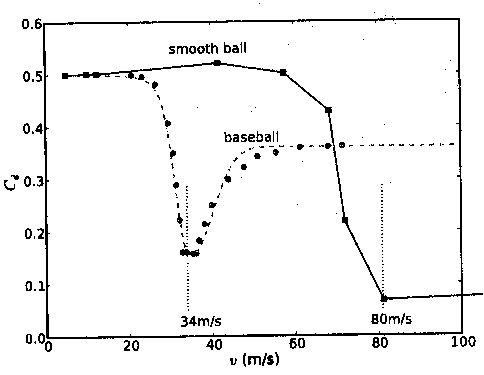
\includegraphics[width=0.6\linewidth]{figs/C_drag_Wang2015.pdf}
    \caption{Drag coefficient $C_D$ as a function of velocity for smooth
      balls (straight line) and baseballs (dashed line). From
      \citet{Wang:2015aa}. Image Copyright \copyright 2015 J.\ Wang.}
    \label{fig:CD}
  \end{figure}
\item Due to friction, the ball will not keep spinning at the initial
  velocity. Instead we can model its slow-down approximately with an exponential
  decay \citep{Nathan:2008aa} (following \citet{Adair:2002aa})
  \begin{gather}
    \label{eq:spinexp}
    \omega(t) = \omega_{0} \exp(-t/\tau).
  \end{gather}
  In principle, $\tau$ is velocity dependent but here you can make the
  simplifying assumption $\tau \approx 5\,\text{s}$ (constant). For
  more details see \citet{Nathan:2008aa}.  
\end{enumerate}

\subsubsection{Tasks}
\label{sec:tasks}

In your analysis show trajectories of pitches with and without the
improved modelling. Comment on the size of the effect.

\begin{enuma}
\item Update the code in \texttt{hw07.py} to include the
  velocity-dependent drag coefficient $C_{D}(v)$ and the slowing down
  of the angular velocity $\omega(t)$. \points{10}
\item Create at least three plots for different choices of the initial
  velocity (which you should choose yourself) where you compare a
  simulation \emph{without} the added effects to one with the effects
  of section \ref{sec:add} included. Analyze your data by briefly
  describing your graphs and commenting on the size of the
  effects. \points{10}
\end{enuma}


\appendix

\section{Baseball physics summary}
\label{sec:curveball}

We want to simulate the trajectory of a \emph{curve ball} in the game
of baseball. In this problem we simplify the problem somewhat to only
include the essential physical effects:
\begin{itemize}
\item Only consider quadratic terms in the air resistance (ignore
  linear terms) and assume that the drag coefficient $b_{2}$ is
  independent of velocity. (See Problem \ref{sec:advanced} below for a
  more realistic approach where $b_{2}(v)$).
\item Consider the \emph{Magnus effect} due to spin but assume that
  the ball spins at constant angular velocity. (See Problem
  \ref{sec:advanced} below for a more realistic approach where the
  angular velocity decays with time.)
\end{itemize}

\paragraph{Quadratic air resistance}

An approximately quadratic dependence of the drag force on the
velocity occurs at high Reynolds numbers, i.e., turbulent flow
(approximately when $\text{Re} > 2300$). An approximate expression
is\footnote{In the Lecture notes we just denoted quadratic drag with
  $\vec{F}_{2} = -b_2 v \vec{v}$ and lumped everything into the
  quadratic drag coefficient $b_{2}$. Eq.~\ref{eq:Fdquadratic} gives
  more physical motivation to $b_{2} = \frac{1}{2} C_{D} \rho A$}
\begin{gather}
\label{eq:Fdquadratic}
  \vec{F}_2 = -\frac{1}{2} C_{D} \rho A v^{2} \frac{\vec{v}}{v}
\end{gather}
We are considering the quadratic drag coefficient $b_{2}$ to be
constant in this problem.

\paragraph{Magnus effect}

The airflow is changed around a spinning object. The Magnus force is
\begin{gather}
  \vec{F}_M = \alpha \boldsymbol{\omega} \times \vec{v}
  \label{eq:Fmagnus}
\end{gather}
where $\boldsymbol{\omega}$ is the ball's angular velocity in rad/s
(e.g., 200/s for a baseball).

For a sphere the proportionality constant $\alpha$ can be written
\begin{gather}
  \vec{F}_M = \frac{1}{2} C_L \rho A \frac{v}{\omega}
  \boldsymbol{\omega} \times \vec{v}\label{eq:sphere}  
\end{gather}
where $C_L$ is the lift coefficient, $\rho$ the air density, $A$ the
ball's cross section. (Advantage of defining $C_L$ this way: when spin
and velocity are perpendicular, the Magnus force is simply
$F_M = \frac{1}{2} C_L \rho A v^2$.)

$C_L$ is mainly a function of the \emph{spin parameter}\footnote{For a
  more detailed discussion that also considers an additional
  $v$-dependence of $C_{L}$ through its dependence on $C_{D}(v)$ see
  \citet{Nathan:2008ac}.}
\begin{gather}
  S = \frac{r\omega}{v}\label{eq:S}  
\end{gather}
with the radius $r$ of the ball. $S = v_{\text{spin}}/v$ is the ratio of the speed of a
point on the ball's surface to the translational speed of the ball. In general we write
\begin{gather}
  \vec{F}_M = \frac{1}{2} C_L \frac{\rho A r}{S}
  \boldsymbol{\omega} \times \vec{v}\label{eq:FM}  
\end{gather}
For a baseball, experimental data show approximately a power law dependence of $C_L$ on $S$
\begin{gather}
  C_L = 0.62 \times S^{0.7}\label{eq:CL}.
\end{gather}

\subsection{Baseball equations}
\label{sec:eq}

In order to simulate the trajectory $\vec{r}(t)$ of a baseball, the
following equations must be solved:
\begin{align}
  \frac{d\vec{r}}{dt} &= \vec{v} \label{eq:drdtv}\\
  \frac{d\vec{v}}{dt} &= -g \hat{\vec{e}}_y  - \frac{b_2}{m} v \vec{v}
          + \frac{\alpha}{m}\ \boldsymbol{\omega} \times \vec{v} \label{eq:dvdta}
\end{align}
with
\begin{gather}
  \label{eq:CD}
  b_{2} = \frac{1}{2} C_{D} \rho A.
\end{gather}
The dependence of the dynamical parameters on spin and velocity is
\begin{align}
  \vec{F}_M &= \alpha\ \boldsymbol{\omega} \times \vec{v}\\
  v &= \sqrt{\vec{v}\cdot\vec{v}} \label{eq:vsquared}\\
  S &= \frac{r\omega}{v}\\
  C_L &= 0.62 \times S^{0.7}\\
  \alpha &= \frac{1}{2} C_L  \frac{\rho A r}{S}
\end{align}

\subsection{Parameters}
\label{sec:parameters}

Use a ball diameter of 7.468~cm, mass of 148.83~g, and a distance of
the pitcher from the home plate $R_\text{homeplate} =
18.4\,\text{m}$.
Use a constant quadratic drag coefficient $C_{D} = 0.40$,
acceleration due to gravity $g = 9.81~\text{m}\cdot\text{s}^{-2}$, and
density of air $\rho = 1.225\,\text{kg}\cdot\text{m}^{-3}$.

% $b_{2} = 0.0013\,\text{N}\cdot\text{s}^{2}\cdot\text{m}^{-2}$

\subsection{Simulation}
\label{sec:sim}

Integrate the equations of motions with the RK4 algorithm
(\texttt{ode.rk4()}). Stop the integration when
$x \ge R_\text{homeplate}$ or $y < 0.2\,\text{m}$
(i.e., cannot be batted). The integration should be performed inside a
function
\begin{minted}{python}
def simulate_baseball(v0, omega, r0,
                      h=0.01, C_D=0.40, g=9.81, rho=1.225,
                      r=0.07468/2, m=0.14883, R_homeplate=18.4):  
\end{minted}
as provided in the skeleton code file \texttt{hw07.py}. As input it
should take the initial velocity vector $\vec{v}_{0}$ (as a 2D array
$(v_{x}, v_{y})$), the ball's rotational velocity vector
$\boldsymbol{\omega}$ (as a 3D array
$(\omega_{x}, \omega_{y}, \omega_{z})$), and the initial position when
leaving the pitcher's hand $\vec{r}_{0} = (x_{0}, y_{0})$ (for
simplicity, set it to $x_{0}=0$ and $y_{0}=2\,\text{m}$).

The function should return the ball's trajectory as an $N \times 4$
array for $N$ time steps along the first axis and
$[t, x(t), y(t), z(t)]$ along the second axis (where $t$ is the time
and the other three entries are the cartesian components of
$\vec{r}(t)$).

\begin{enuma}
\item Simulate a horizontal baseball throw for initial velocity
  $\vec{v} = (30\,\text{m/s}, 0)$.  Try out different spins; a good
  starting value is
  $\boldsymbol{\omega} = 200\,\text{rad/s} \times (0, 1, 1)$. In
  particular, simulate the baseball throw with
  \begin{enumi}
  \item almost no spin: $\omega = 0.001 \times (0, 0, 1)$ (our code
    does not handle $\omega = 0$ gracefully...)
  \item $\omega = 200 \times (0, 0, 1)$
  \item $\omega = 200 \times (0, 1, 1)$
  \end{enumi}
\item Plot the three scenarios in 2D planes: $x$-$y$ (side view) and
  $x$-$z$ (top view). Plot all throws together and add a
  legend. Briefly describe and discuss the trajectories.
\item Plot in 3D (see Appendix \ref{sec:mpl}).
\end{enuma}


\section{3D plotting with matplotlib}
\label{sec:mpl}

For the 3D-plotting you can use \texttt{matplotlib} as described in
the
\href{http://matplotlib.org/mpl_toolkits/mplot3d/tutorial.html}{mplot3d
  Tutorial}. In the \emph{jupyter} notebook you can enable
interactive view where you can rotate the 3D plot
\begin{minted}{python}
%matplotlib notebook
\end{minted}
For using \texttt{matplotlib} for 3D graphs you need to import
\texttt{Axes3D} as shown below and then use the
\texttt{projection='3d'} keyword argument for \texttt{add\_subplot()}.
\begin{minted}{python}
import matplotlib.pyplot as plt
from mpl_toolkits.mplot3d import Axes3D
fig = plt.figure()
ax = fig.add_subplot(1,1,1, projection='3d')

# add plots for multiple throws: note the order
# of the coordinates
ax.plot(X, Z, Y, 'o', label="no spin")

ax.set_xlabel("$x$ (m)")
ax.set_ylabel("$z$ (m)")
ax.set_zlabel("$y$ (m)")
ax.legend(loc="upper left", numpoints=1)
ax.figure.tight_layout()
\end{minted}

\bibliographystyle{physbiol-natbib}      % basic style, author-year citations with url
\bibliography{assignment_07}

\end{document}

%%% Local Variables: 
%%% mode: latex
%%% TeX-master: t
%%% End: 
